\documentclass[12pt,answers]{exam}

\usepackage{amsmath,amsfonts,amssymb,mathtools,physics,commath}
\usepackage{todonotes}
\usepackage{float}
\usepackage{multicol}

\newcommand{\inv}{^{-1}}

\pagestyle{headandfoot}
\firstpageheadrule
\runningheadrule
\firstpageheader{Math 221}{Exam 1|Solutions, Page \thepage\ of \numpages}{February 4, 2020}
\runningheader{Math 221}{Exam 1|Solutions, Page \thepage\ of \numpages}{February 4, 2020}
\runningfooter{}{}{}

\begin{document}
% \maketitle
\begin{questions}
	\question
	Evaluate the following integrals.
	\begin{parts}
		\part[10]
		$\displaystyle \int \frac{\sin(\sqrt x)}{\sqrt x} \dif x$
		\begin{solution}
			Let $u = \sqrt x$, so $\dif u = \dfrac{1}{2\sqrt x} \dif x$.
			Then
			\begin{align*}
				\int \frac{\sin(\sqrt x)}{\sqrt x} \dif x
				 & = 2 \int \sin u \dif u         \\
				 & = -2 \cos u                    \\
				 & = \boxed{-2 \cos(\sqrt x) + C}
			\end{align*}
		\end{solution}
		\part[10]
		$\displaystyle \int \frac{x}{\sqrt{x+1}} \dif x$
		\begin{solution}
			Letting $u = x + 1$, so $\dif u = \dif x$ and $u-1 = x$
			Then
			\begin{align*}
				\int \frac{x}{\sqrt{x+1}} \dif x
				 & = \int \frac{u-1}{\sqrt u} \dif u                \\
				 & = \int u^{1/2} - u^{-1/2}                        \\
				 & = \frac23 u^{3/2} - 2u^{1/2}                     \\
				 & = \boxed{\frac23 (x+1)^{3/2} - 2(x+1)^{1/2} + C}
			\end{align*}
		\end{solution}
	\end{parts}

\newpage
\question
Evaluate the following integrals.
\begin{parts}
	\part[10]
	$\displaystyle \int \sin\inv x \dif x$, where $\sin\inv x$ is the inverse sine function.
	\begin{solution}
		IBP:
		\[
			\begin{array}{ccc}
				  & D                       & I \\
				+ & \sin\inv x              & 1 \\
				- & \dfrac{1}{\sqrt{1-x^2}} & x
			\end{array}
		\]
		so
		\begin{align*}
			\int \sin\inv x \dif x
			 & = x \sin \inv x - \int \frac{x}{\sqrt{1-x^2}}  \qquad (u = 1-x^2; \dif u = -2x \dif x) \\
			 & = x \sin \inv x + \frac12 \int \frac{1}{\sqrt{u}} \dif u                               \\
			 & = x \sin \inv x + u^{1/2}                                                              \\
			 & = \boxed{x \sin \inv x + \sqrt{1-x^2} + C}
		\end{align*}
	\end{solution}

	\part[10]
	$\displaystyle \int x^7 \ln x \dif x$,
	\begin{solution}
		IBP:
		\[
			\begin{array}{ccc}
				  & D        & I             \\
				+ & \ln x    & x^7           \\
				- & \dfrac 1x & \dfrac{x^8}{8}
			\end{array}
		\]
		so
		\begin{align*}
			\int x^7 \ln x \dif x
			 & = \frac{x^8}{8} \ln x - \int \frac 18 x^7 \dif x     \\
			 & = \boxed{\frac{x^8}{8} \ln x - \frac{1}{64} x^8 + C}
		\end{align*}
	\end{solution}
\end{parts}

\newpage
\question
Evaluate the following integrals.
\begin{parts}
	\part[10]
	$\displaystyle \int_0^{\pi/4} \sin(4x)\sin(2x)\dif x$.
	Express your final answer as a reduced fraction $\dfrac ab$, with no trig functions.
	\begin{solution}
		Starting with the sum-to-product formula on the cover page,
		\begin{align*}
			\int_0^{\pi/4} \sin(4x)\sin(2x)\dif x
			 & = \frac12 \int_0^{\pi/4} \cos(2x) - \cos(6x) \dif x                             \\
			 & = \frac 12 \left[\frac12 \sin(2x) - \frac 16 \sin(6x)\right]_0^{\pi/4}          \\
			 & = \frac 12 \left[\frac12 \sin(\frac\pi2) - \frac 16 \sin(\frac{3\pi}{2})\right] \\
			 & = \frac 12 \left[\frac12 + \frac 16\right]                                      \\
			 & = \boxed{\frac 13}
		\end{align*}
	\end{solution}
	\part[10]
	$\displaystyle \int \frac{\dif x}{\sqrt{4+x^2}}$
	\begin{solution}
		Trig sub: $x = 2 \tan \theta$, so $\dif x = 2 \sec^2 \theta \dif \theta$,
		\begin{multicols}{2}
			\begin{align*}
				\int \frac{\dif x}{\sqrt{4+x^2}}
				 & = \int \frac{2\sec^2 \theta \dif \theta}{\sqrt{4+4\tan^2 \theta}}   \\
				 & = \int \frac{2\sec^2 \theta \dif \theta}{\sqrt{4(1+\tan^2 \theta)}} \\
				 & = \int \frac{2\sec^2 \theta \dif \theta}{2\sqrt{\sec^2 \theta}}     \\
				 & = \int \sec \theta \dif \theta                                      \\
				 & = \ln|\sec \theta + \tan \theta |                                   \\
				 & = \boxed{\ln \left| \frac{\sqrt{x^2+4}}{2} + \frac x2\right| + C}
			\end{align*}
			\begin{figure}[H]
				\centering
				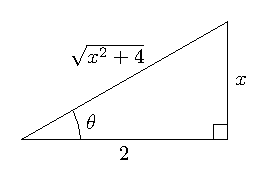
\includegraphics{graphics/2020-spring-exam1-3b.pdf}
			\end{figure}
		\end{multicols}
	\end{solution}
\end{parts}

\newpage
\question Evaluate the following integrals.
\begin{parts}
	\part[10] $\displaystyle \int \sin[4](x) \cos[7](x) \dif x$
	\begin{solution}
		\begin{align*}
			\int \sin[4](x) \cos[7](x) \dif x 
			& = \int \sin[4](x) \underbracket{\cos[6](x)}_{(\cos^2(x))^3} \cos x \dif x \\ 
			&= \int \sin[4](x) \underbracket{(1-\sin[2](x))^3}_{\substack{\text{rewritten with } \\ \cos^2 = 1-\sin^2}} \cos x \dif x \\ 
			&= \int u^4 (1-u^2)^3 \dif u \\ 
			&= \int u^4 (1 - 3 u^2 + 3 u^4 - u^6) \dif u \\ 
			&= \int u^4 - 3u^6 + 3u^8 - u^{10} \dif u \\ 
			&= \frac{u^5}{5} - \frac37 u^7 + \frac13 u^9 - \frac{1}{11} u^{11} \\ 
			&= \boxed{\frac15 \sin^5(x) - \frac37 \sin^7(x) + \frac13 \sin^9(x) - \frac{1}{11} \sin^{11}(x) + C}
		\end{align*}
	\end{solution}
	\part[10] $\displaystyle \int \sec[4](x) \dif x$
	\begin{solution}
		Using reduction formula on cover page:
		\begin{align*}
			\int \sec[4](x) \dif x 
			= \frac{\sec[2](x)\tan(x)}{3} + \frac23 \int \sec[2](x) \dif x  \\ 
			= \boxed{\frac{\sec[2](x)\tan(x)}{3} + \frac23 \tan x + C}
		\end{align*}
	\end{solution}
\end{parts}

\newpage
\question[10]
An object moves along a straight line with velocity function $v(t) = t \sin t$, in meters per second. Determine its change in position over the time interval $t = 0$ to $t = \pi$ seconds. (Evaluate any trig function in your answer.)
\begin{solution}
	The object's displacement is given by the integral $\displaystyle \int_0^\pi t \sin t \dif t$.
	Evaluating this uses IBP:
	\[
		\begin{array}{ccc}
			& D & I \\ 
			+ & t & \sin t \\ 
			- & 1 & -\cos t \\ 
			+ & 0 & -\sin t
		\end{array}
	\]
	Thus
	\[
		\int_0^\pi t \sin t \dif t
		= \eval{-t \cos t + \sin t}_0^\pi
		= \pi - 0 = \boxed{\pi \text{ meters}}
	\]
\end{solution}

% \newpage
\question[10]
Find a function $f(t)$ such that $f'(t) = \dfrac{\ln t}{t} - \cos(2\pi t)$.
\begin{solution}
	\begin{align*}
		\int \left( \dfrac{\ln t}{t} - \cos(2\pi t) \right)\dif t
		= \boxed{\frac12 (\ln t)^2 - \frac{1}{2\pi} \sin(2\pi t) + C}
	\end{align*}
	(The first term is integrated with $u=\ln t$. The second term can be done with $u=2\pi t$, though it is also a guess-and-fudge type of $u$-sub.)
\end{solution}
\end{questions}
\end{document}
